\chapter{Project}

\section{Code Concept}

In extend to this article a code base is available \footnote{\url{https://www.github.com/florianwiech/incremental-machine-learning}}.
This code base includes the reimplementation of EWC and the extension of modifying the Fisher information matrix.
It uses Python 3 with the packages NumPy (version 1.16.1) and Tensorflow (version 1.13.0).
The concept documents the code structure and procedure.

The complete code consists of three files.
"main.py", "network.py" and "mnist.py".

\begin{figure}[H]
    \centering
    
\includegraphics[scale=.4]{project/concept/files}
    \caption{File structure}
    \label{fig:concept_file_structure}
\end{figure}

The "\textbf{mnist.py}" makes the MNIST dataset available.
It loads the MNIST database automatically, reshapes the values and data structures and splits or permutes the dataset if neccesary.
After the calculation, it returns the arrays in Python standard datastructures with the extension of multi-dimensional arrays from NumPy.
\newline
"\textbf{network.py}" holds the "Network" class.
The class consists of all neccesary operations for the EWC algorithm with original and adaption.
The contructor creates a neural network with 784 input neurons, three hidden layers with 800 neurons each and the ten MNIST output classes.
In addition to that, it initializes all neccesary functions like loss and accuracy.
After the initialization, the object offers several methods for training, testing and applying EWC to the task.
Figure \ref{fig:concept_class_diagram} shows a class diagram of the Network class.

\begin{figure}[H]
    \centering
    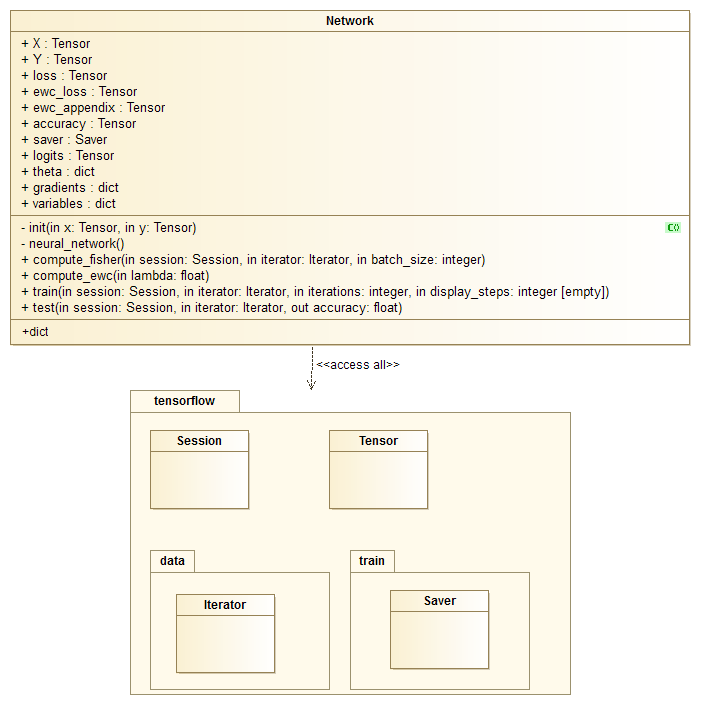
\includegraphics[scale=.6]{project/concept/class_diagram}
    \caption{Class diagram}
    \label{fig:concept_class_diagram}
\end{figure}

During execution, the network occupies multiple states.
The states distinguish if the network trains the first task or loads a previous state and retrains the network.
Figure \ref{fig:concept_state_diagram} shows the state diagram for the network:

\begin{figure}[H]
    \centering
    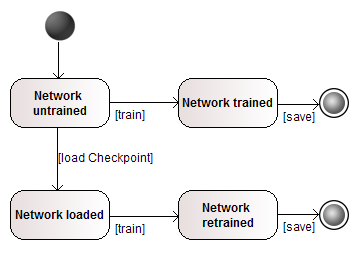
\includegraphics[scale=.8]{project/concept/state_diagram}
    \caption{State diagram}
    \label{fig:concept_state_diagram}
\end{figure}

"\textbf{main.py}" is the entrypoint of the code base.
It offers a command line tool for specification of the neccesary parameters.
\newline
The main function executes one task and saves their state in a checkpoint.
If the executed task is the first task, the network gets initialized.
In this case the EWC appendix in the loss funtion is not applied.
The network gets trained, the matrix gets calculated and the final model with matrix calculation is saved in a checkpoint.
For each following ongoing task the main file has to be restarted with new args values.
In these cases the network will be initialized with the EWC loss function.
The new created Tensorflow session restores a checkpoint given by the parameter (checkpoint of the task before) and the network gets retrained.

The sequential execution is shown in a sequence diagram.
The first part (Figure \ref{fig:concept_sequence_diagram_part_1}) shows the initialization of all neccesary parameters and objects.
Part 2 (Figure \ref{fig:concept_sequence_diagram_part_2}) shows the execution of training and testing the neural network.

\begin{figure}[H]
    \centering
    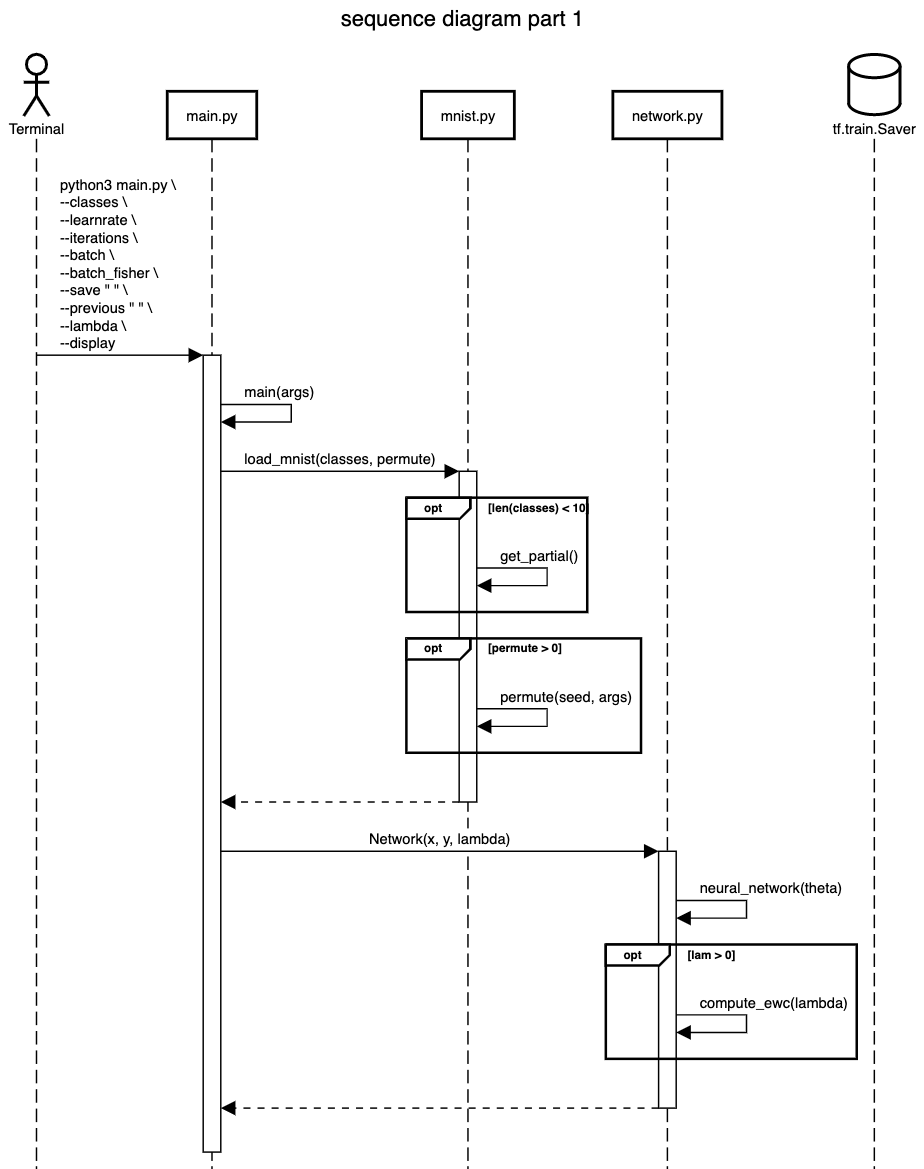
\includegraphics[width=\textwidth]{project/concept/sequence_diagram_part_1}
    \caption{Sequence diagram part 1}
    \label{fig:concept_sequence_diagram_part_1}
\end{figure}

\begin{figure}[H]
    \centering
    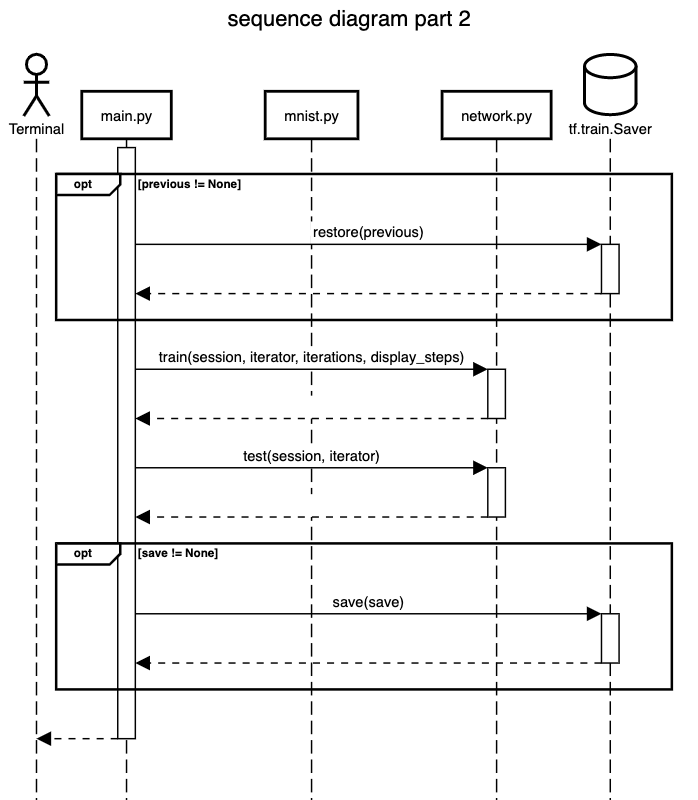
\includegraphics[width=\textwidth]{project/concept/sequence_diagram_part_2}
    \caption{Sequence diagram part 2}
    \label{fig:concept_sequence_diagram_part_2}
\end{figure}

\newpage
\section{Baseline}

Before adapting the EWC algorithm, the codebase has to proof that it delivers the results of the EWC paper.
The original EWC algorithm is tested in the constructed benchmarks described in Project Goals (Section \ref{project_goals}):

\subsection{Disjoint 9-1 Benchmark}

$T_1$, trained with the classes zero to eight, reaches an accuracy of 95.72\% at the end of its training period.
The task was trained with a learning rate of 0.001, 2,500 iterations and a batch size of 100.
In comparison to the complete dataset (green, line), the accuracy is 86.06\%.

$T_2$ trained with the class nine further of $T_1$ uses a learning rate of 0.00001, 2,500 iterations and a batch size of 100.
The lambda value is $\frac{1}{0.00001} = 100,000$.
It reaches an accuracy of 97.81\%.

At the end of $T_2$ trainng phase designates $T_1$ to 84.50\% and the complete dataset 85.44\%.
The complete dataset reaches a peak of 93.43\% where $T_1$ has 94.87\% precision and $T_2$ 76.66\% precision.

Figure \ref{fig:ewc_d9-1} shows the trainings of both tasks compared to the accuracy of the complete dataset:

\begin{figure}[H]
    \centering
    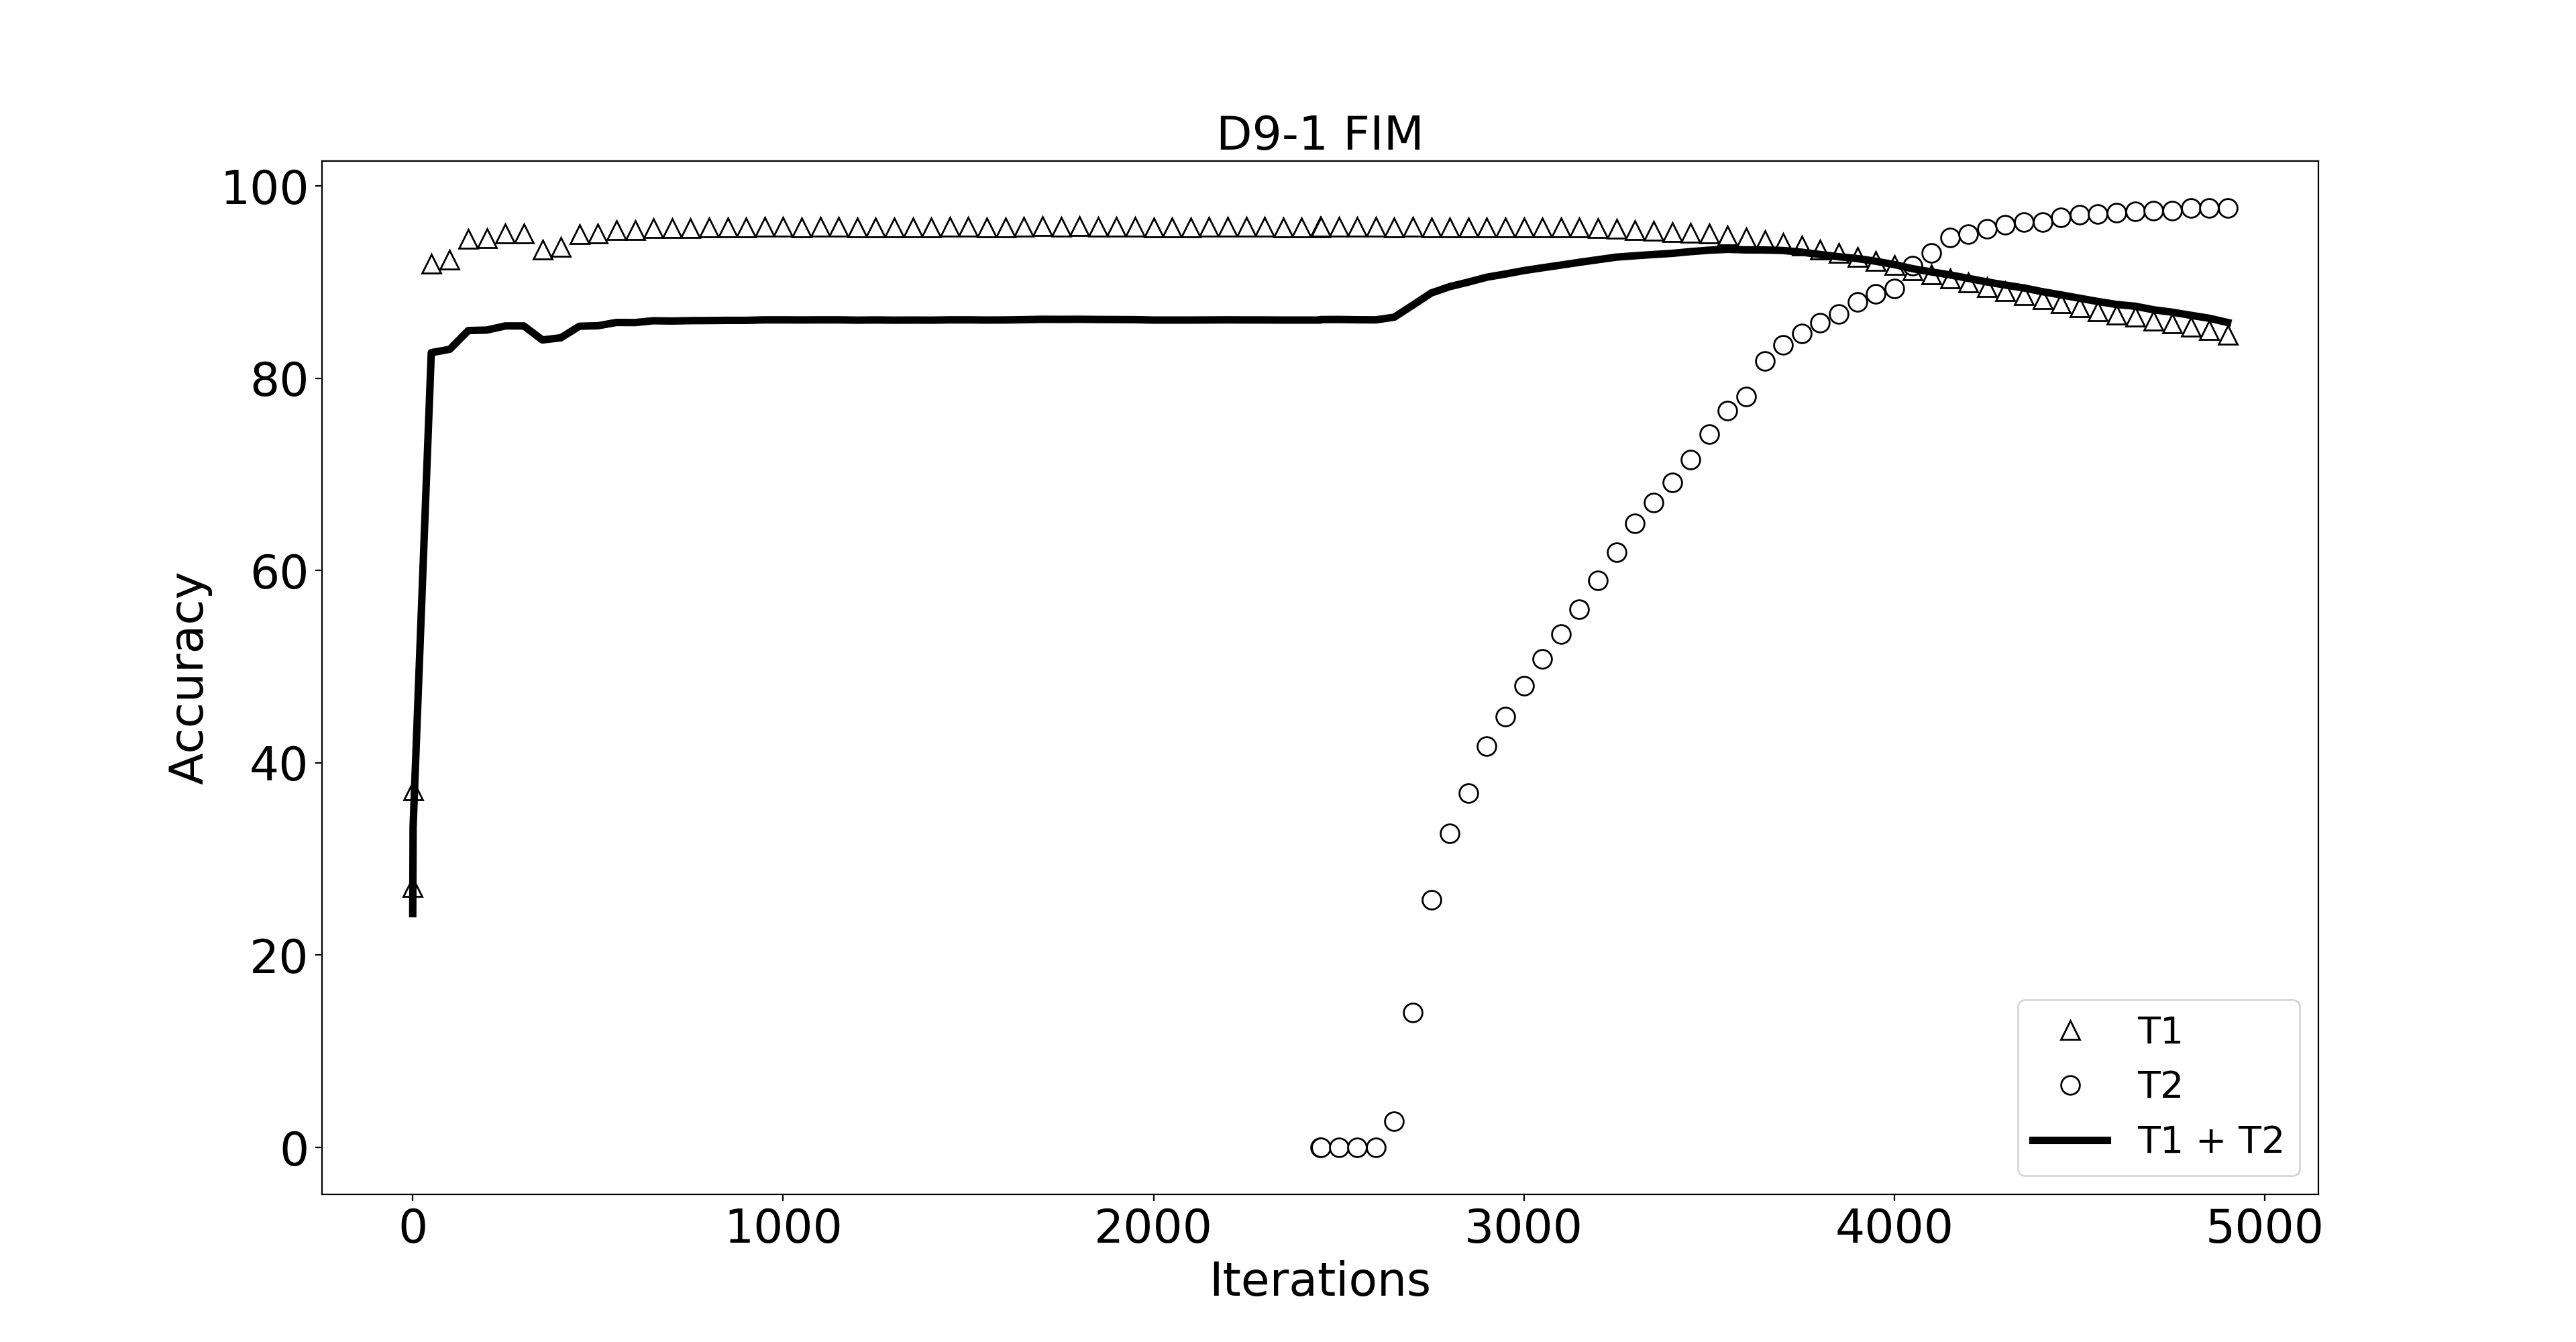
\includegraphics[width=\textwidth]{project/baseline/D91_FIM}
    \caption{EWC D9-1}
    \label{fig:ewc_d9-1}
\end{figure}

\subsection{Disjoint 5-5 Benchmark}

Figure \ref{fig:ewc_d5-5} shows training of a disjoint MNIST with a five class split.

The first Task $T_1$ with the classes zero to four reaches an accuracy of 98.66\% after the first training.
$T_1$ was trained with a learning rate of 0.001, 2,500 iterations and a batch size of 100.
Since there are only five of ten possible classes trained, the accuracy on the complete dataset amounts 50.70\%.

In the second training period with task $T_2$, the classes five to nine achieve an accuracy of 82.67\%.
The learning rate of $T_2$ is 0.00001 and there were again 2,500 iterations and a batch size of 100.
Since it is an ongoing task, the EWC appendix is applied to the loss.
In this case lambda was set to $\frac{1}{0.00001} = 100,000$.

After the second training, $T_1$ lost 22.22\%, but still shows a quality of 76.44\%.
The performance of the complete dataset ascended from 50.70\% to 79.39\%.

\begin{figure}[H]
    \centering
    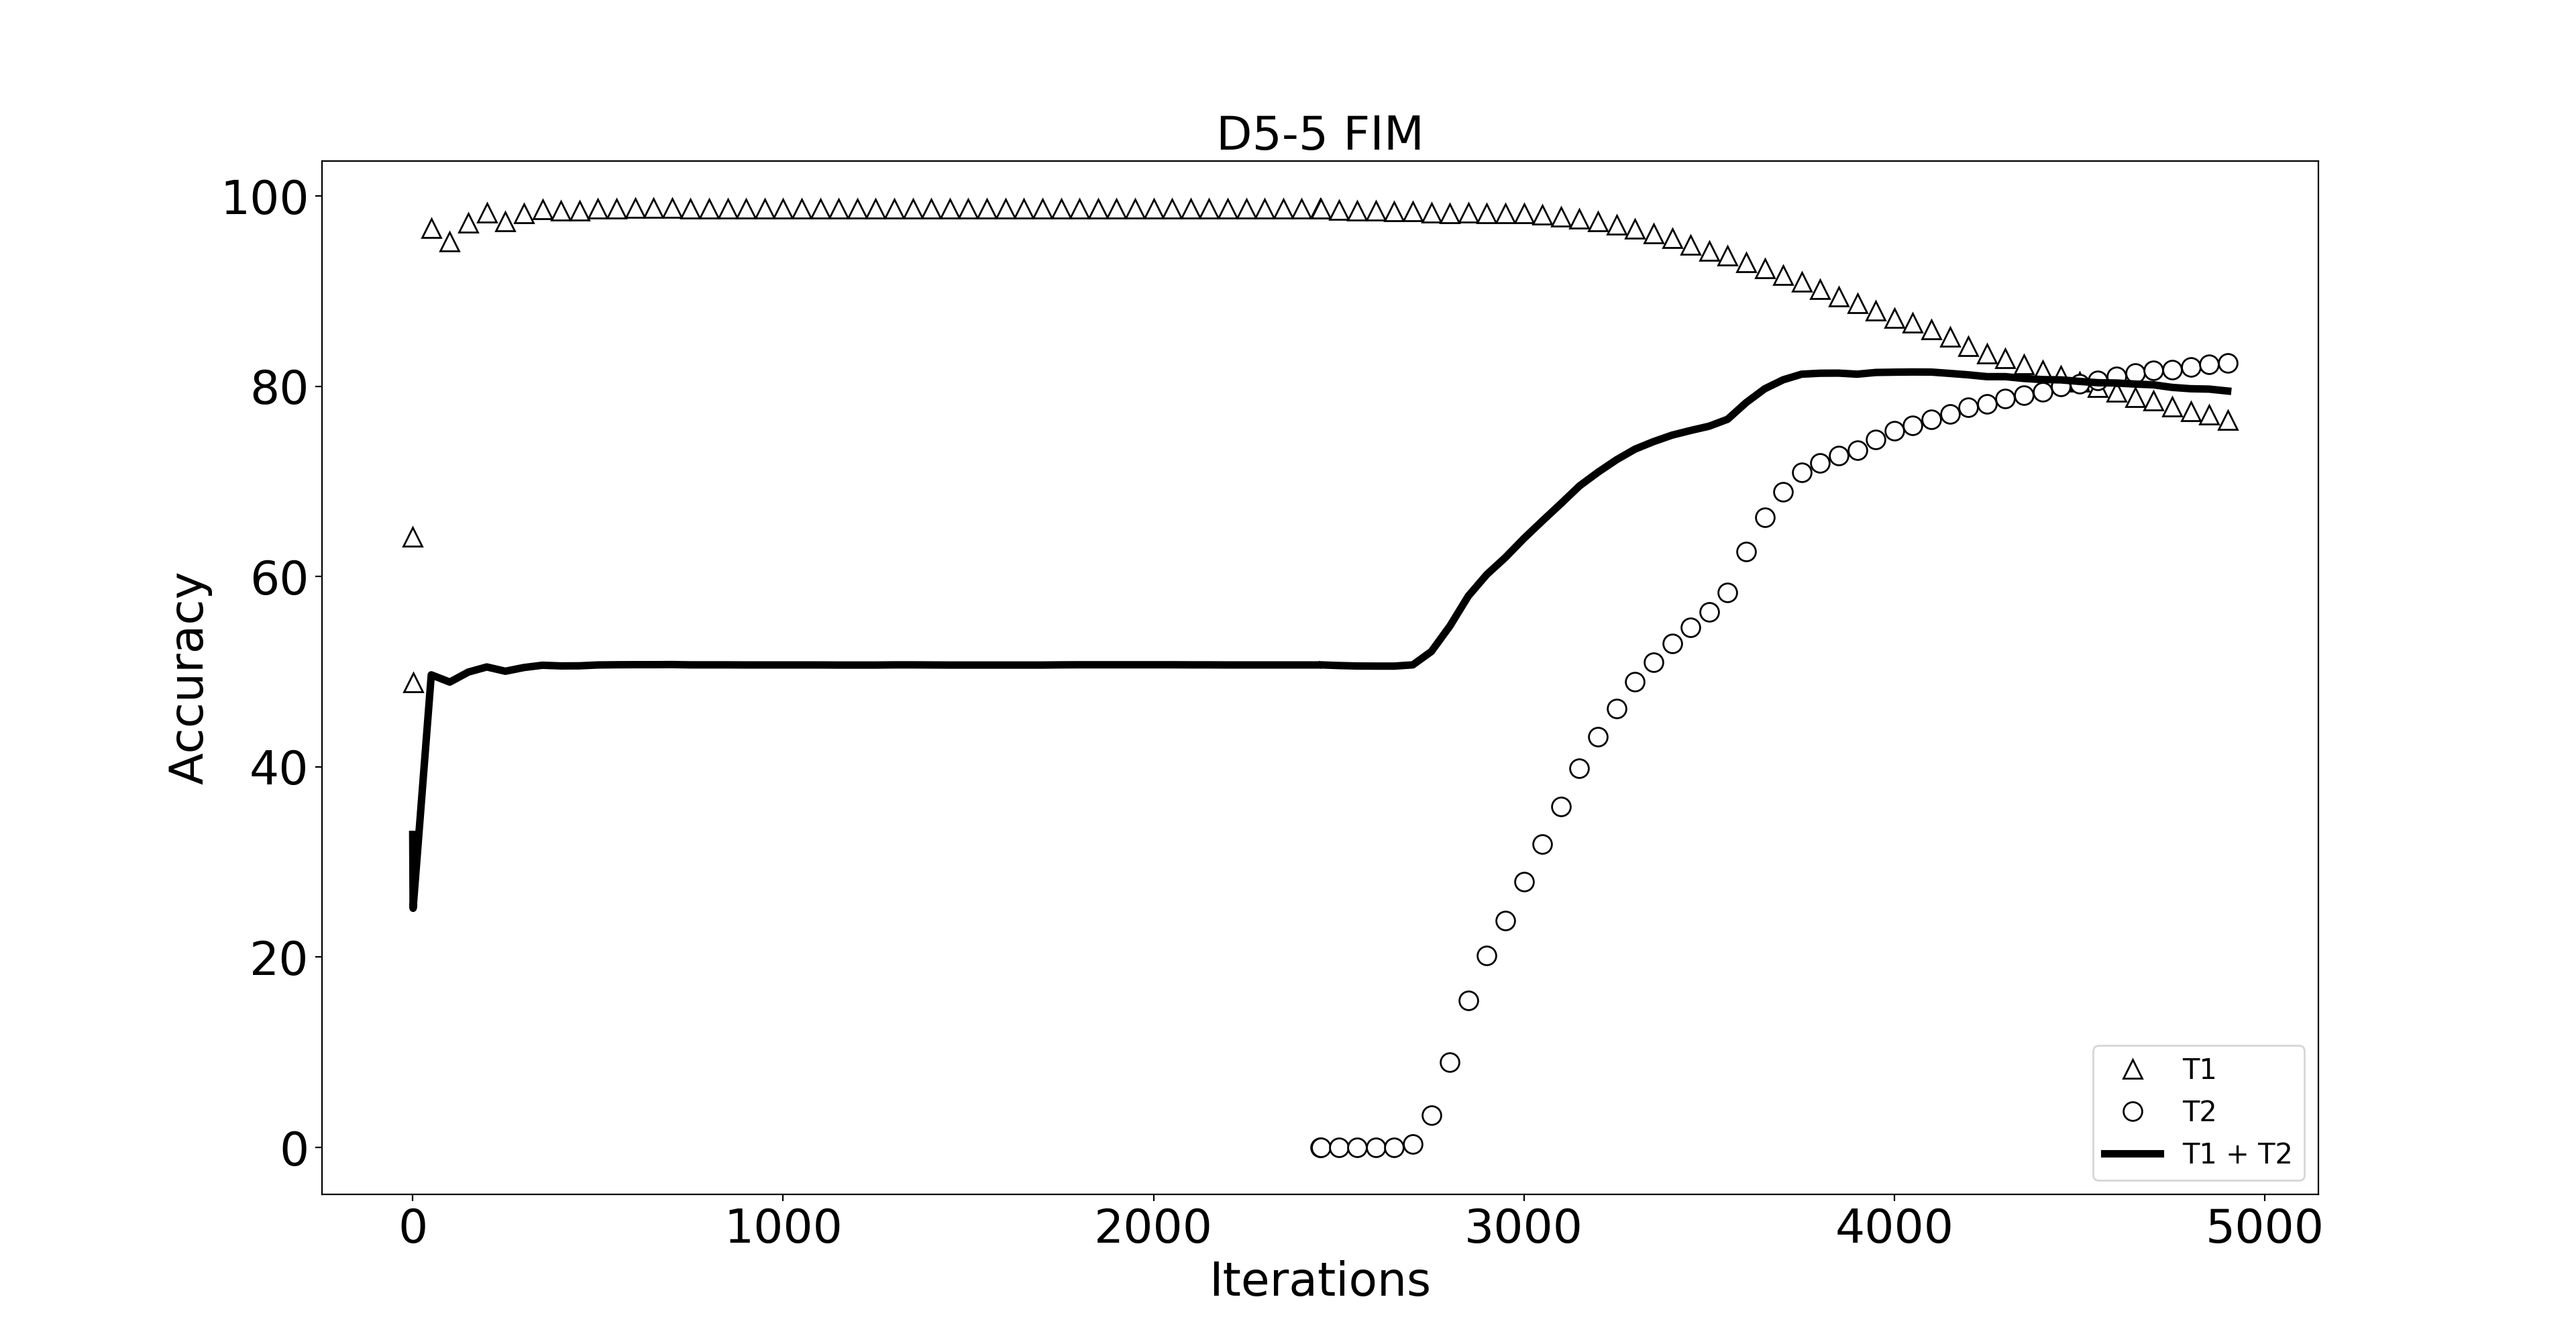
\includegraphics[width=\textwidth]{project/baseline/D55_FIM}
    \caption{EWC D5-5}
    \label{fig:ewc_d5-5}
\end{figure}

\subsection{Permuted 10-10 Benchmark}

EWC performance is shown in Figure \ref{fig:ewc_p10-10}.
$T_1$ is trained with following parameters:
all classes with a
learning rate of 0.001,
60,000 samples,
batch size of 100 in
2,500 iterations.
After the $T_1$ training, it shows an accuracy of 94.76\% which is equally to the complete dataset.
\newline
$T_2$ on the other hand learned with a rate of 0.00001 with 20,000 iterations.
The 60,000 samples were permuted with a seed of zero and split into batches with a size of 100.
The importance of the EWC loss was $\lambda = \frac{1}{0.00001} = 100,000$.
$T_2$ needed in this case a longer learning rate to be able to have a good accuracy.
It shows a performance of 91.45\% and 90.53\% on the complete dataset.
$T_1$ still performs with 94.78\%.

\begin{figure}[H]
    \centering
    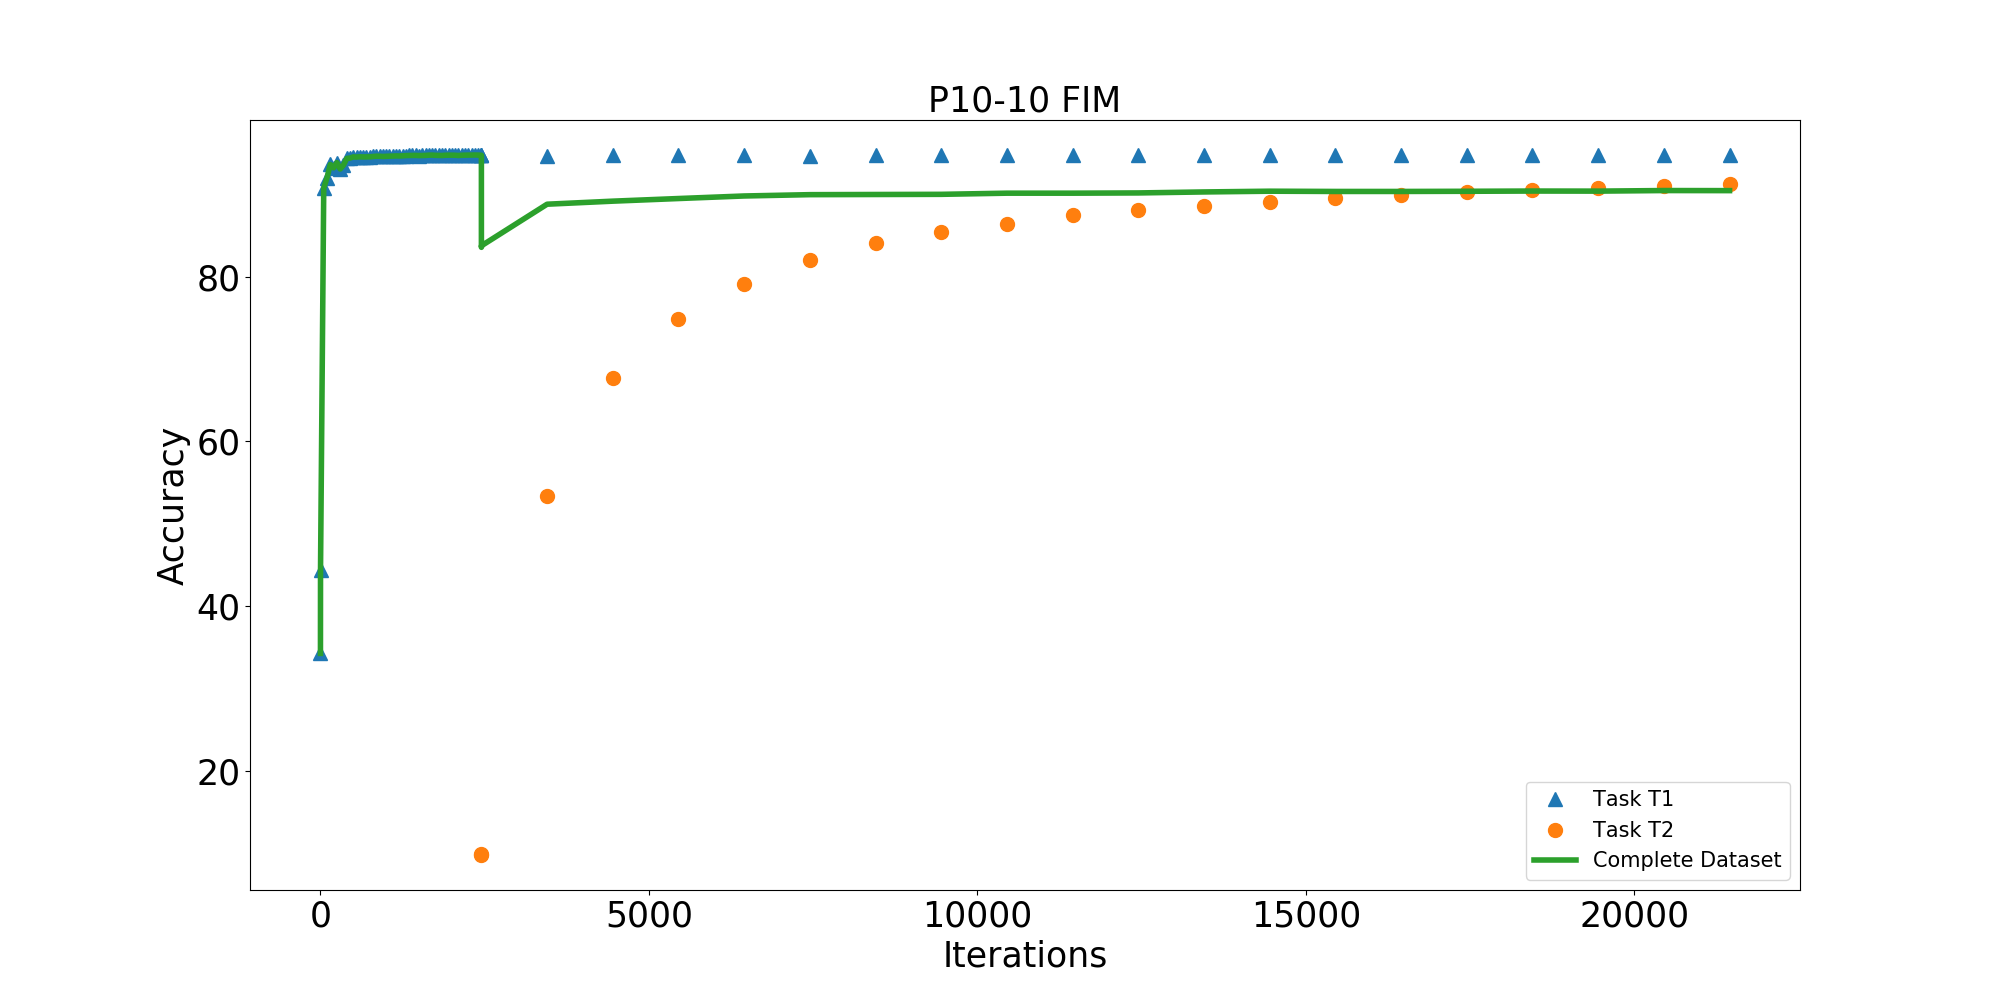
\includegraphics[width=\textwidth]{project/baseline/P10-10_FIM_IT20k}
    \caption{EWC P10-10}
    \label{fig:ewc_p10-10}
\end{figure}

\newpage

\section{Critical review of EWC and improvements}
\label{project_review_improvements}

The EWC loss function uses the original loss function with the EWC appendix:

\begin{equation}
    \mathcal{L} = 
    \mathcal{L}^{CE} 
    + \sum_{i} 
        \frac{\lambda}{2} 
        F_{i} 
        (\theta_{i} - \theta_{T_1,i}^{*})^2
\end{equation}

For a better understanding can the abstract parameter $\theta$ split into the explicit weight and bias parameters.
The weights are represented as $W^i$ vectors and the biases as $B^i$ vectors, where the index $i$ is for each layer, $i \in \{ 0, \dots, L-1 \}$.
The EWC term has the following notation:

\begin{equation}
    \begin{split}
        \mathcal{L} = \mathcal{L}^{CE}
        & + \frac{\lambda}{2} \sum_{i=0}^{L-1} \sum_{k, l} F_{k, l}^{W^i}\left(W^i_{k, l}-W^{i,{T_1}}_{k, l} \right)^2
        \\
        & +  \frac{\lambda}{2}\sum_{i=0}^{L-1} \sum_{k}F^{B^i}_k\left(B^i_{k}-B^{i,{T_1}}_{k} \right)^2
    \end{split}
\end{equation}

As proposed in Elastic Weight Consolidation (Section \ref{foundation_ewc}, \cite{elastic-weight-consolidation}) the authors use the Fisher information matrix for the loss calculation. It is calculated over all training samples:

\begin{equation}
    F_{ij} = 
    \frac{1}{N} 
    \sum_{n=1}^{N} 
    \left(
        \frac{\partial \mathcal{L} \left( x_n \right) }{\partial \theta_{i}} 
        \cdot 
        \frac{\partial \mathcal{L} \left( x_n \right) }{\partial \theta_{j}}
    \right)
\end{equation}

In fact it is only the diagonal of the Fisher information matrix:

\begin{equation}
    \begin{split}
        \vec{F} & = diag \left( F_{ij} \right)
        \\
        F_{j} & = 
        \frac{1}{N} 
        \sum_{n=1}^{N} 
        \left(
            \frac{\partial \mathcal{L} \left( x_n \right) }{\partial \theta_{j}}
        \right)^2
    \end{split}
\end{equation}

This matrix equation calculates an average over all training samples N.
As well as the EWC term, it can be split into the weight and bias vectors:

\begin{equation}
    \begin{split}
        \vec{F}^{W^i}_j & = 
        \frac{1}{N} 
        \sum_{n=1}^{N} 
        \left(
            \frac{\partial \mathcal{L} \left( x_n \right) }{\partial W^i_{j}}
        \right)^2
        \\
        \vec{F}^{B^i}_j & = 
        \frac{1}{N} 
        \sum_{n=1}^{N} 
        \left(
            \frac{\partial \mathcal{L} \left( x_n \right) }{\partial B^i_{j}}
        \right)^2
    \end{split}
\end{equation}

The reports \cite{better-weight-consolidation,elastic-weight-consolidation} justify that the assumption of the diagonal FIM is common practice \cite{elastic-weight-consolidation,better-weight-consolidation,incremental-moment-matching}.
It reduces the operations from $O(N^2)$ to $O(N)$, where $N$ is the number of elements in $\theta$ \cite{elastic-weight-consolidation,better-weight-consolidation}.
This reulsts in a lot faster calculation even in large models \cite{elastic-weight-consolidation,better-weight-consolidation}.
Moreover, this justification receives rather promising results and holds in some cases.
\cite{elastic-weight-consolidation,incremental-moment-matching}.

So the main justificaion for the diagonal FIM seems to be the rather promising results.
\newline
This article tries another calculation on the EWC loss, that is not based on diagonal assumptions, but with a mathematical principle.
\newline
A closer look to the EWC appendix shows, that the term $(\theta_i - \theta^*_{T_1,i})^2$ calculates the divergence between the new calculated parameters and the parameters of the old task.
With the square they are made positive.
At this point is the original algorithm multiplied by the diagonal FIM, which provides the importance.
So this article wants to find a way to measure the importance of the parameters.
Here this article fills the gap with the first derivative of the loss by the parameters.
The understanding of the first derivative is the slope of every parameter.
So a change of the higher gradients compared to the other parameters would bring the network faster out of balance.
And this is, what EWC algorithm wants to protect. Their goal is it to stay as close as possible to the old important parameters and just adjust the ones with less importance.
The first derivative of the loss with the parameters over all training samples of a batch N:

\begin{equation}
    \begin{split}
        \mathcal{L}_k & = 
        \frac{1}{N}
        \sum_{n} 
            \mathcal{L}(x_n)
        \\
        \frac{\partial \mathcal{L}(x_n)}{\partial \theta_k} & = 
        \frac{1}{N}
        \sum_{n} 
            \frac{\partial \mathcal{L}(x_n)}{\partial \theta_k}
    \end{split}
\end{equation}

This first derivative gets squared to positive all results and bring the parameters into a higher value space.
This operation is allowd, because the important factor in the matrix is the ranking between the values, which will not be changed.

\begin{equation}
    \left[
        \frac{\partial \mathcal{L}(x_n)}{\partial \theta_k}
        \right]^2
    = 
    \left[
        \frac{1}{N}
        \sum_{n} 
            \frac{\partial \mathcal{L}(x_n)}{\partial \theta_k}
        \right]^2
\end{equation}

So the calculated matrix with the new approach is shown in Equation \eqref{eq:gradient_matrix}.

\begin{equation}
    \mathcal{F}_k =
    \left(
        \frac{1}{N}
        \sum_{n} 
            \frac{\partial \mathcal{L}(x_n)}{\partial \theta_k}
        \right)^2
    \label{eq:gradient_matrix}
\end{equation}

This matrix calculated the first derivation over all the training samples $N$ in each batch
Since $\theta$ only consists of weight and bias vectors, it can be re-arrange for the two matrices:

\begin{equation}
    \begin{split}
        \vec{F}^{W^i}_j & = 
        \left(
            \frac{1}{N} 
            \sum_{n=1}^{N}
            \frac{\partial \mathcal{L} \left( x_n \right) }{\partial W^i_{j}}
        \right)^2
        \\
        \vec{F}^{B^i}_j & = 
        \left(
            \frac{1}{N} 
            \sum_{n=1}^{N} 
            \frac{\partial \mathcal{L} \left( x_n \right) }{\partial B^i_{j}}
        \right)^2
    \end{split}
\end{equation}

% then: its is similiar to the orginial gradient but not the same -> show formula
% clarifythe problem with tensorflow and that this equation is not the gradient

For convenience this article uses the shorthand "GM" (Gradient Matrix) for the new matrix operation.
\newline
The comparison between FIM and GM shows that their similar, but not the same for $N > 1$.
The FIM uses the square of the first derivation of each sample. GM on the other hand takes the gradient of a training set (batch) as an importance indicator and squares it for a positive result.
However, in the case of $N=1$, the Gradient Matrix is identical to the FIM.
$N=1$ means that the training set (batch) only contains one sample.

The current reference implementation \footnote[1]{\url{https://github.com/ariseff/overcoming-catastrophic}} of EWC uses Tensorflow.
A problem with calculating the FIM in Tensorflow is that it is neccesary to get the gradients for every sample but Tensorflow does not expose them.
So the reference implementation built a complex workaround by hardcoding the gradients directly into the computation graph of Tensorflow.
This increases the memory consumption by the batch size.
It results that the developer set the batch size for this computation to the fixed rate of 100, because the computation of a full batch would directly run out of memory.
\cite{github_ewc_issue_one}
The new matrix in contrast squares the gradient after averaged, which solves this problem.

The following section tests this modification on the D9-1, D5-5 and P10-10 benchmarks.

\newpage
\section{Experimental Results}

This following section shows the results of EWC with the Gradient matrix.
It tests several parameter values.
Mainly the learning rate and lambda are varied.
The network features are listed in Section \ref{foundations_deep_neural_network}.

\subsection{Disjoint 9-1}

% TODO first sentence
All experiments with a disjoint nine to one test on MNIST are split in the task $T_1$ with numbers zero to eight and task $T_2$ with number nine.
Task $T_1$ was trained on 54,000 samples, split into batches with a size of 100.
The learning rate amounted 0.001.
The calculation of the modified FIM was done with a batch size of 1,000.
This reults in a performance of 95.72\% on the $T_1$ testset and 86.06\% on the complete set.

Besides, Figure \ref{fig:exp_d9-1_bs1k} shows the training of $T_1$ the retraining of the network with $T_2$.
$T_2$ included 5900 samples that were split into 59 batches and tarined in 2,500 iterations.
The learning rate of the optimizer was 0.00001 and $\lambda = \frac{1}{0.00001} = 100,000$.
$T_2$ achives a performance of 97.72\%.
At the end of both trainings $T_1$ performs with 83.60\%.
The complete testset indicates an accuracy of 84.72\%, a minus of 1.34\%.

\begin{figure}[H]
    \centering
    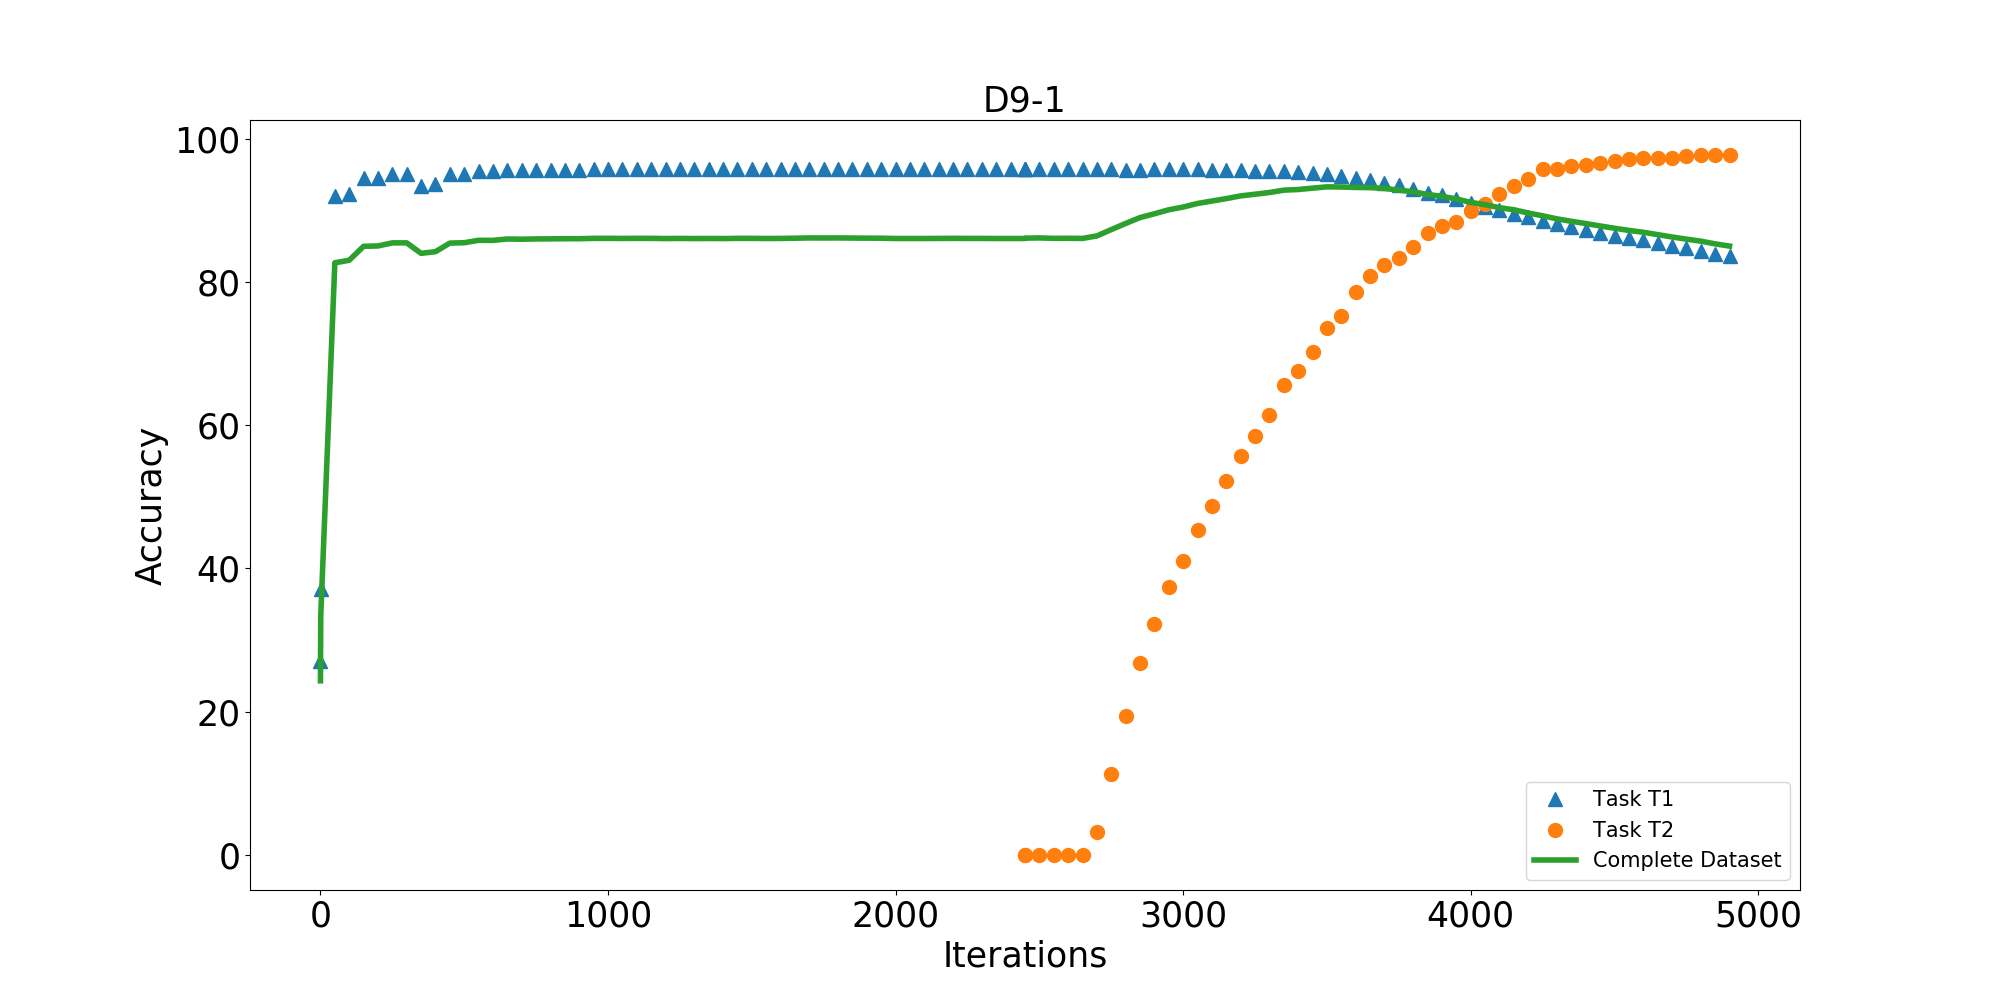
\includegraphics[width=\textwidth]{project/experiments/D91_BS1k}
    \caption{Experiment D9-1}
    \label{fig:exp_d9-1_bs1k}
\end{figure}

\newpage

Table \ref{table:exp_d9-1} tests multiple learning rates and lambda values with $T_2$ on the complete dataset.
Every parameter test was done with 2,500 iterations and a batch size of 100 and 5900 samples.
\newline
The results show that the best performance is with a learning rate of 0.00001 and a lambda value of 1,000,000.
With these parameters $T_2$ performs 87.78\%, $T_1$ still has a performance of 74.12\% and the complete dataset of 90.84\%.

\begin{table}[H]
    \centering
    \begin{tabular}{ |c|l|l|l|  }
        \hline
        \multicolumn{2}{|c|}{parameters} & \multicolumn{2}{c|}{accuracy after $T_2$ training} \\
        \hline
        learning rate & lambda & $T_2$ & complete dataset\\
        \hline
        \hline
        \multirow{6}{*}{0.001} & 1,000 & 100\% & 11.20\%\\
                            & 10,000 & 100\% & 12.78\%\\
                            & 100,000 & 100\% & 12.93\% \\
                            & 1,000,000 & 100\% & 15.92\% \\
                            & 1,010,000 & 100\% & 15.14\% \\
                            & 1,050,000 & 100\% & 14.65\% \\
        \hline
        \multirow{6}{*}{0.0001} & 1,000 & 100\% & 42.22\%\\
                                & 10,000 & 100\% & 40.47\%\\
                                & 100,000 & 100\% & 37.86\% \\
                                & 1,000,000 & 100\% & 41.99\% \\
                                & 1,010,000 & 100\% & 40.09\% \\
                                & 1,050,000 & 100\% & 40.11\% \\
        \hline
        \multirow{6}{*}{0.00001} & 1,000 & 98.91\% & 82.62\%\\
                                & 10,000 & 98.82\% & 83.48\%\\
                                & 100,000 & 97.82\% & 85.41\% \\
                                & 1,000,000 & 87.78\% & 90.84\% \\
                                & 1,010,000 & 87.69\% & 90.86\% \\
                                & 1,050,000 & 87.51\% & 90.87\% \\
        \hline
        \multirow{6}{*}{0.000001} & 1,000 & 94.27\% & 90.2\% \\
                                & 10,000 & 80.34\% & 92.81\% \\
                                & 100,000 & 3.18\% & 86.4\% \\
                                & 1,000,000 & 0.0\% & 86.17\% \\
                                & 1,010,000 & 0.0\% & 86.16\% \\
                                & 1,050,000 & 0.0\% & 86.16\% \\
        \hline
    \end{tabular}
    \caption{Experiment D9-1}
    \label{table:exp_d9-1}
\end{table}

\newpage

\subsection{Disjoint 5-5}

% TODO anfang verbessern (+zeiten)
The disjoint 5-5 experiments a split into the first class with the numbers zero to four and second class with the numbers five to nine.
$T_1$ has 30,500 samples split into 305 batches and trained with 2,500 batch cycles.
The learning rate is 0.001, which results in a $T_1$ performance of 98.66\% and 50.70\% on the complete dataset.
The matric calculation for the second task was done with an average gradient of 1,000 gradients.

Figure \ref{fig:exp_d5-5_bs1k} show both tasks $T_1$ and $T_2$.
In this case $T_2$ was trained with 29,400 samples, a batch size of 100 and a learning rate of 0.00001.
The EWC loss was calculated with $\lambda = \frac{1}{0.00001} = 100,000$.
The result of $T_2$ training is a performance of 82.30\% on $T_2$, 76.73\% on $T_1$ and an accuracy of 79.33\% on the complete dataset.
This shows that the network achvieved an increase of 28.63\%.

\begin{figure}[H]
    \centering
    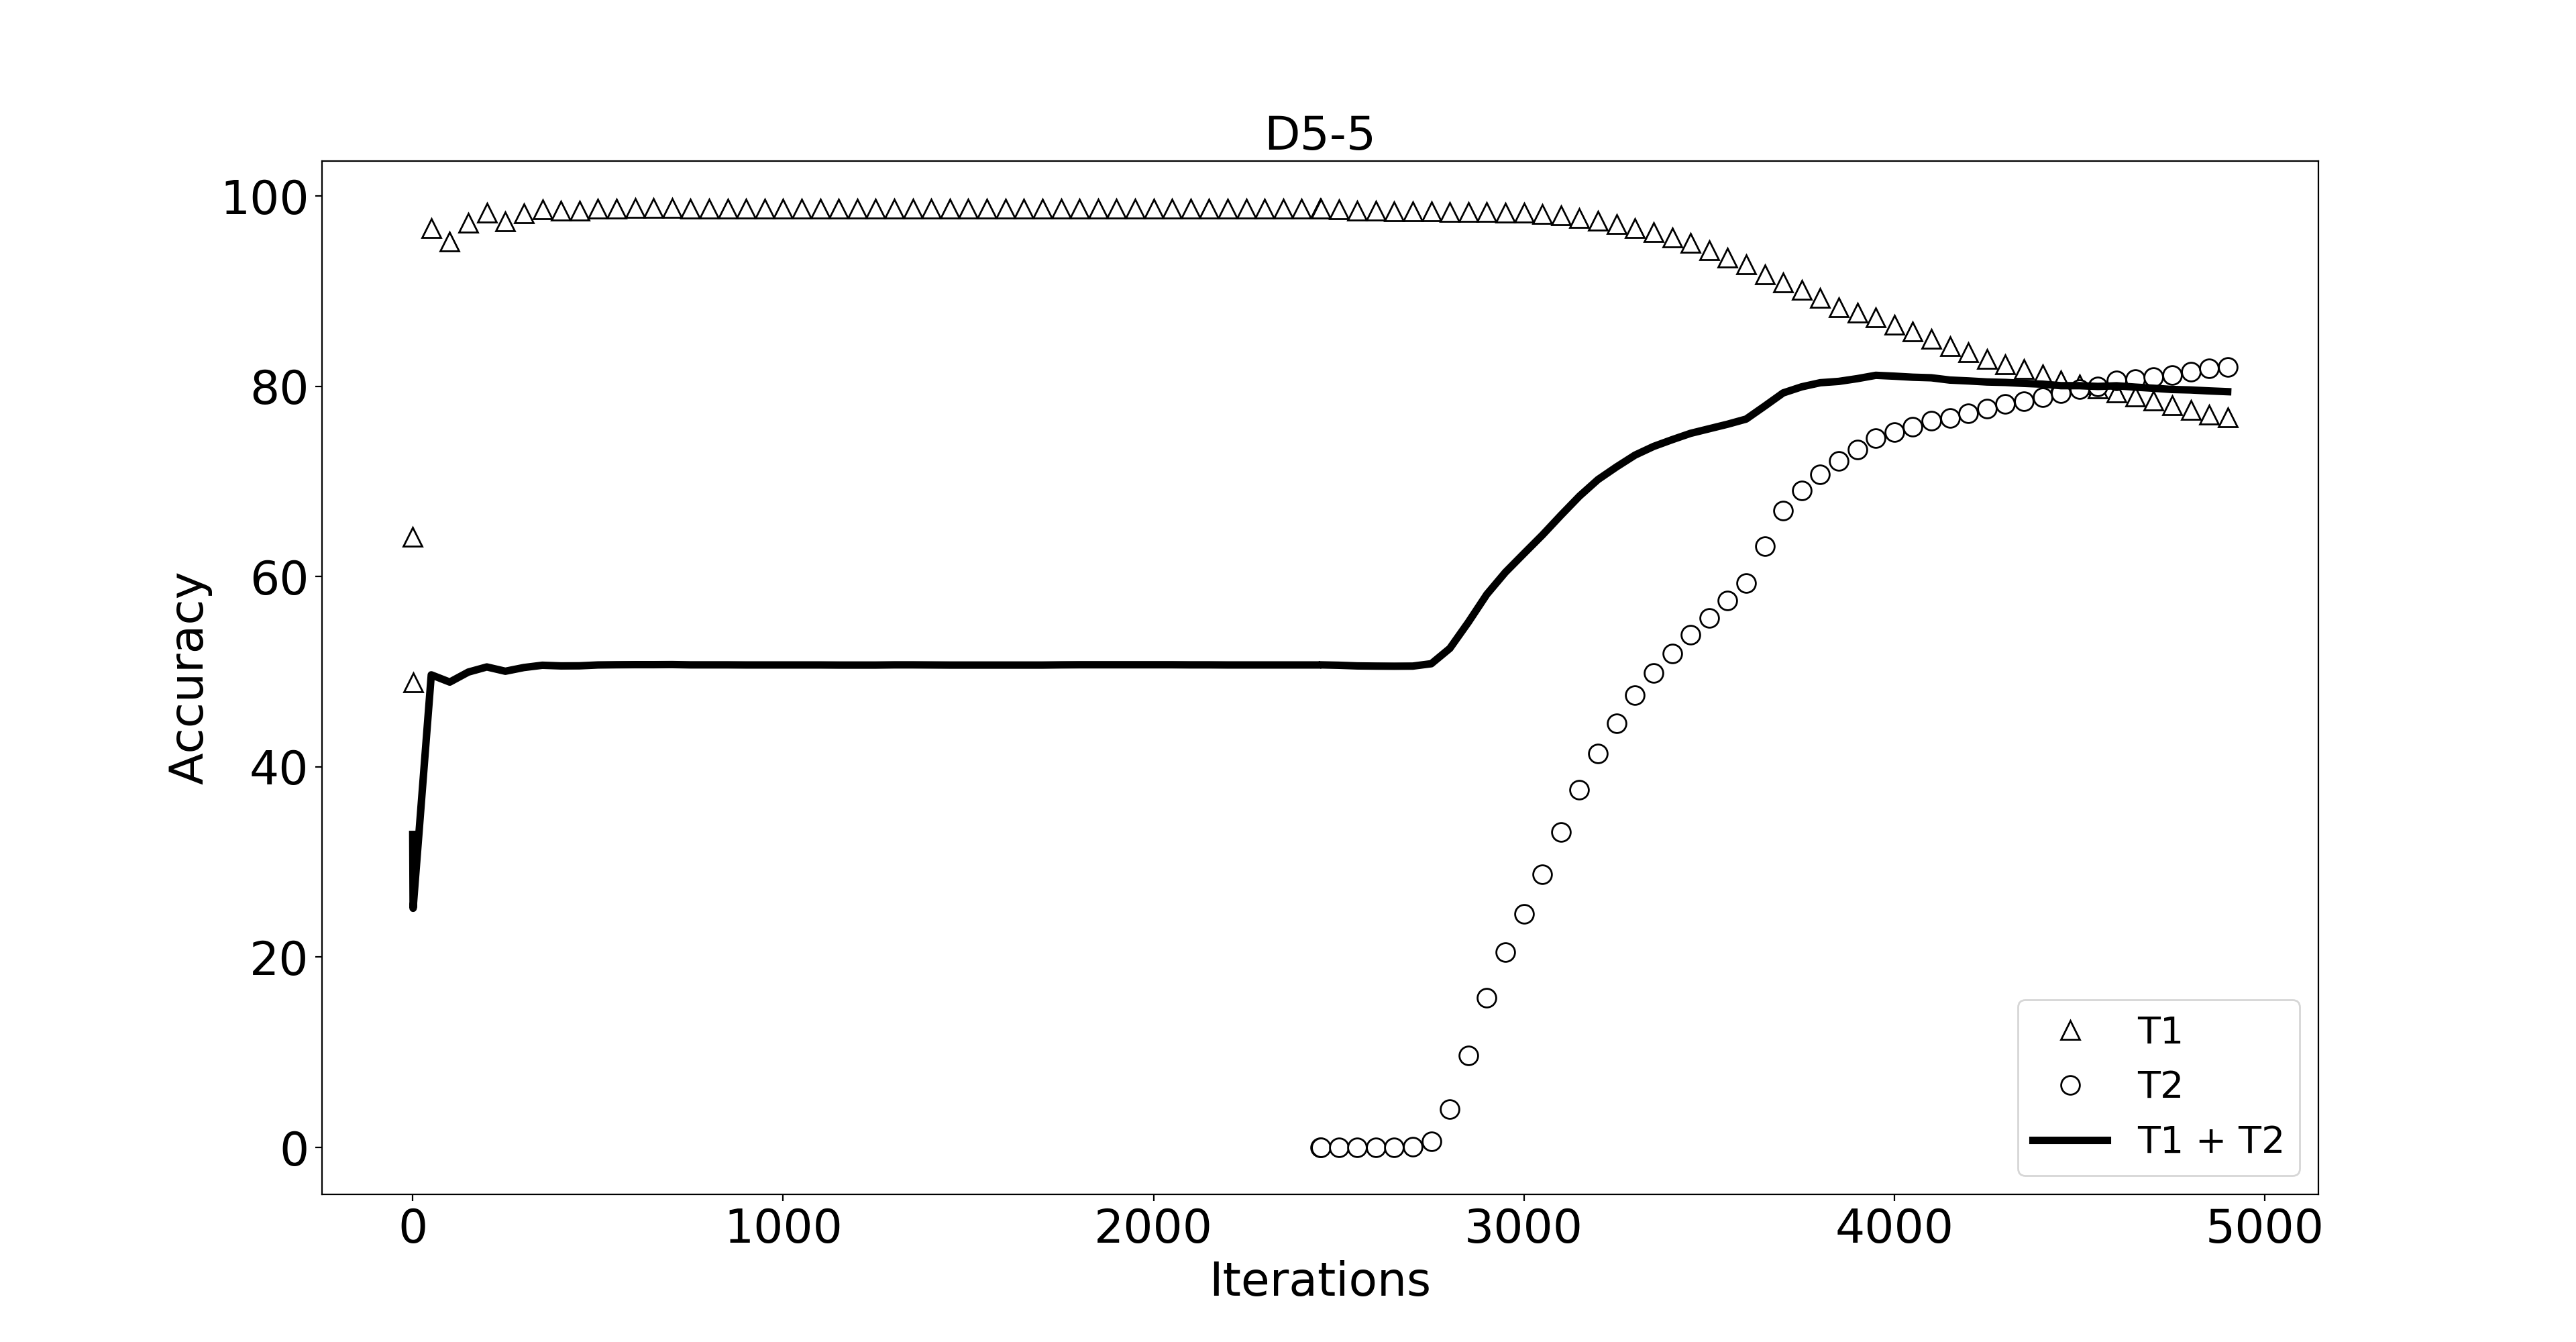
\includegraphics[width=\textwidth]{project/experiments/D55_BS1k}
    \caption{Experiment D-5}
    \label{fig:exp_d5-5_bs1k}
\end{figure}

\newpage

Table \ref{table:exp_d5-5} lists several parameter tests.
These tests are built with the same parameters for $T_2$ except of the learning rate and lambda.
The results are based on a varied learning rate and lambda value.
The best result is with the learning rate of 0.00001 and a lambda value of 1,000.
It shows that the complete set has an accuracy of 81.87\%, $T_2$ of 93.64\% and $T_1$ of 71.16\%.

\begin{table}[H]
    \centering
    \begin{tabular}{ |c|l|l|l|  }
        \hline
        \multicolumn{2}{|c|}{parameters} & \multicolumn{2}{c|}{accuracy after $T_2$ training} \\
        \hline
        learning rate & lambda & $T_2$ & complete dataset\\
        \hline
        \hline
        \multirow{6}{*}{0.001} & 1,000 & 97.87\% & 48.94\%\\
                            & 10,000 & 98.13\% & 49.84\%\\
                            & 100,000 & 97.94\% & 51.04\% \\
                            & 1,000,000 & 97.5\% & 51.72\% \\
                            & 1,010,000 & 97.27\% & 51.99\% \\
                            & 1,050,000 & 97.52\% & 52.75\% \\
        \hline
        \multirow{6}{*}{0.0001} & 1,000 & 97.05\% & 63.24\%\\
                                & 10,000 & 96.65\% & 63.49\%\\
                                & 100,000 & 96.19\% & 61.74\% \\
                                & 1,000,000 & 95.65\% & 63.14\% \\
                                & 1,010,000 & 95.74\% & 63.06\% \\
                                & 1,050,000 & 95.59\% & 63.03\% \\
        \hline
        \multirow{6}{*}{0.00001} & 1,000 & 93.64\% & 81.87\%\\
                                & 10,000 & 90.45\% & 83.49\%\\
                                & 100,000 & 82.38\% & 79.86\% \\
                                & 1,000,000 & 67.84\% & 72.68\% \\
                                & 1,010,000 & 67.79\% & 72.64\% \\
                                & 1,050,000 & 67.2\% & 72.42\% \\
        \hline
        \multirow{6}{*}{0.000001} & 1,000 & 28.1\% & 63.55\% \\
                                & 10,000 & 18.9\% & 59.39\% \\
                                & 100,000 & 0.02\% & 50.6\% \\
                                & 1,000,000 & 0.0\% & 50.71\% \\
                                & 1,010,000 & 0.0\% & 50.71\% \\
                                & 1,050,000 & 0.0\% & 50.71\% \\
        \hline
    \end{tabular}
    \caption{Experiment D5-5}
    \label{table:exp_d5-5}
\end{table}

\newpage

\subsection{Permuted 10-10}

This experiment type performs in $T_1$ a training on the complete dataset and in $T_2$ on a permuted dataset with the random seed of zero.
\newline
$T_1$ properties are: 60,000 samples into 60 batches with a size of 100, a learning rate of 0.001 and 2,500 iterations.
This results in an accuracy of 94.76\%.
The matrix calculation fot the EWC loss used a batch size of 1,000.
\newline
This experiment was as well as the baseline trained with 20,000 iterations on $T_2$.
The change of the learning rate to 0.00001 and $\lambda = \frac{1}{0.00001} = 100,000$, $T_2$ achives a performance of 91.53\%.
The complete dataset shows an accuracy of 90.45\% and $T_1$ of still 94.76\%.

\begin{figure}[H]
    \centering
    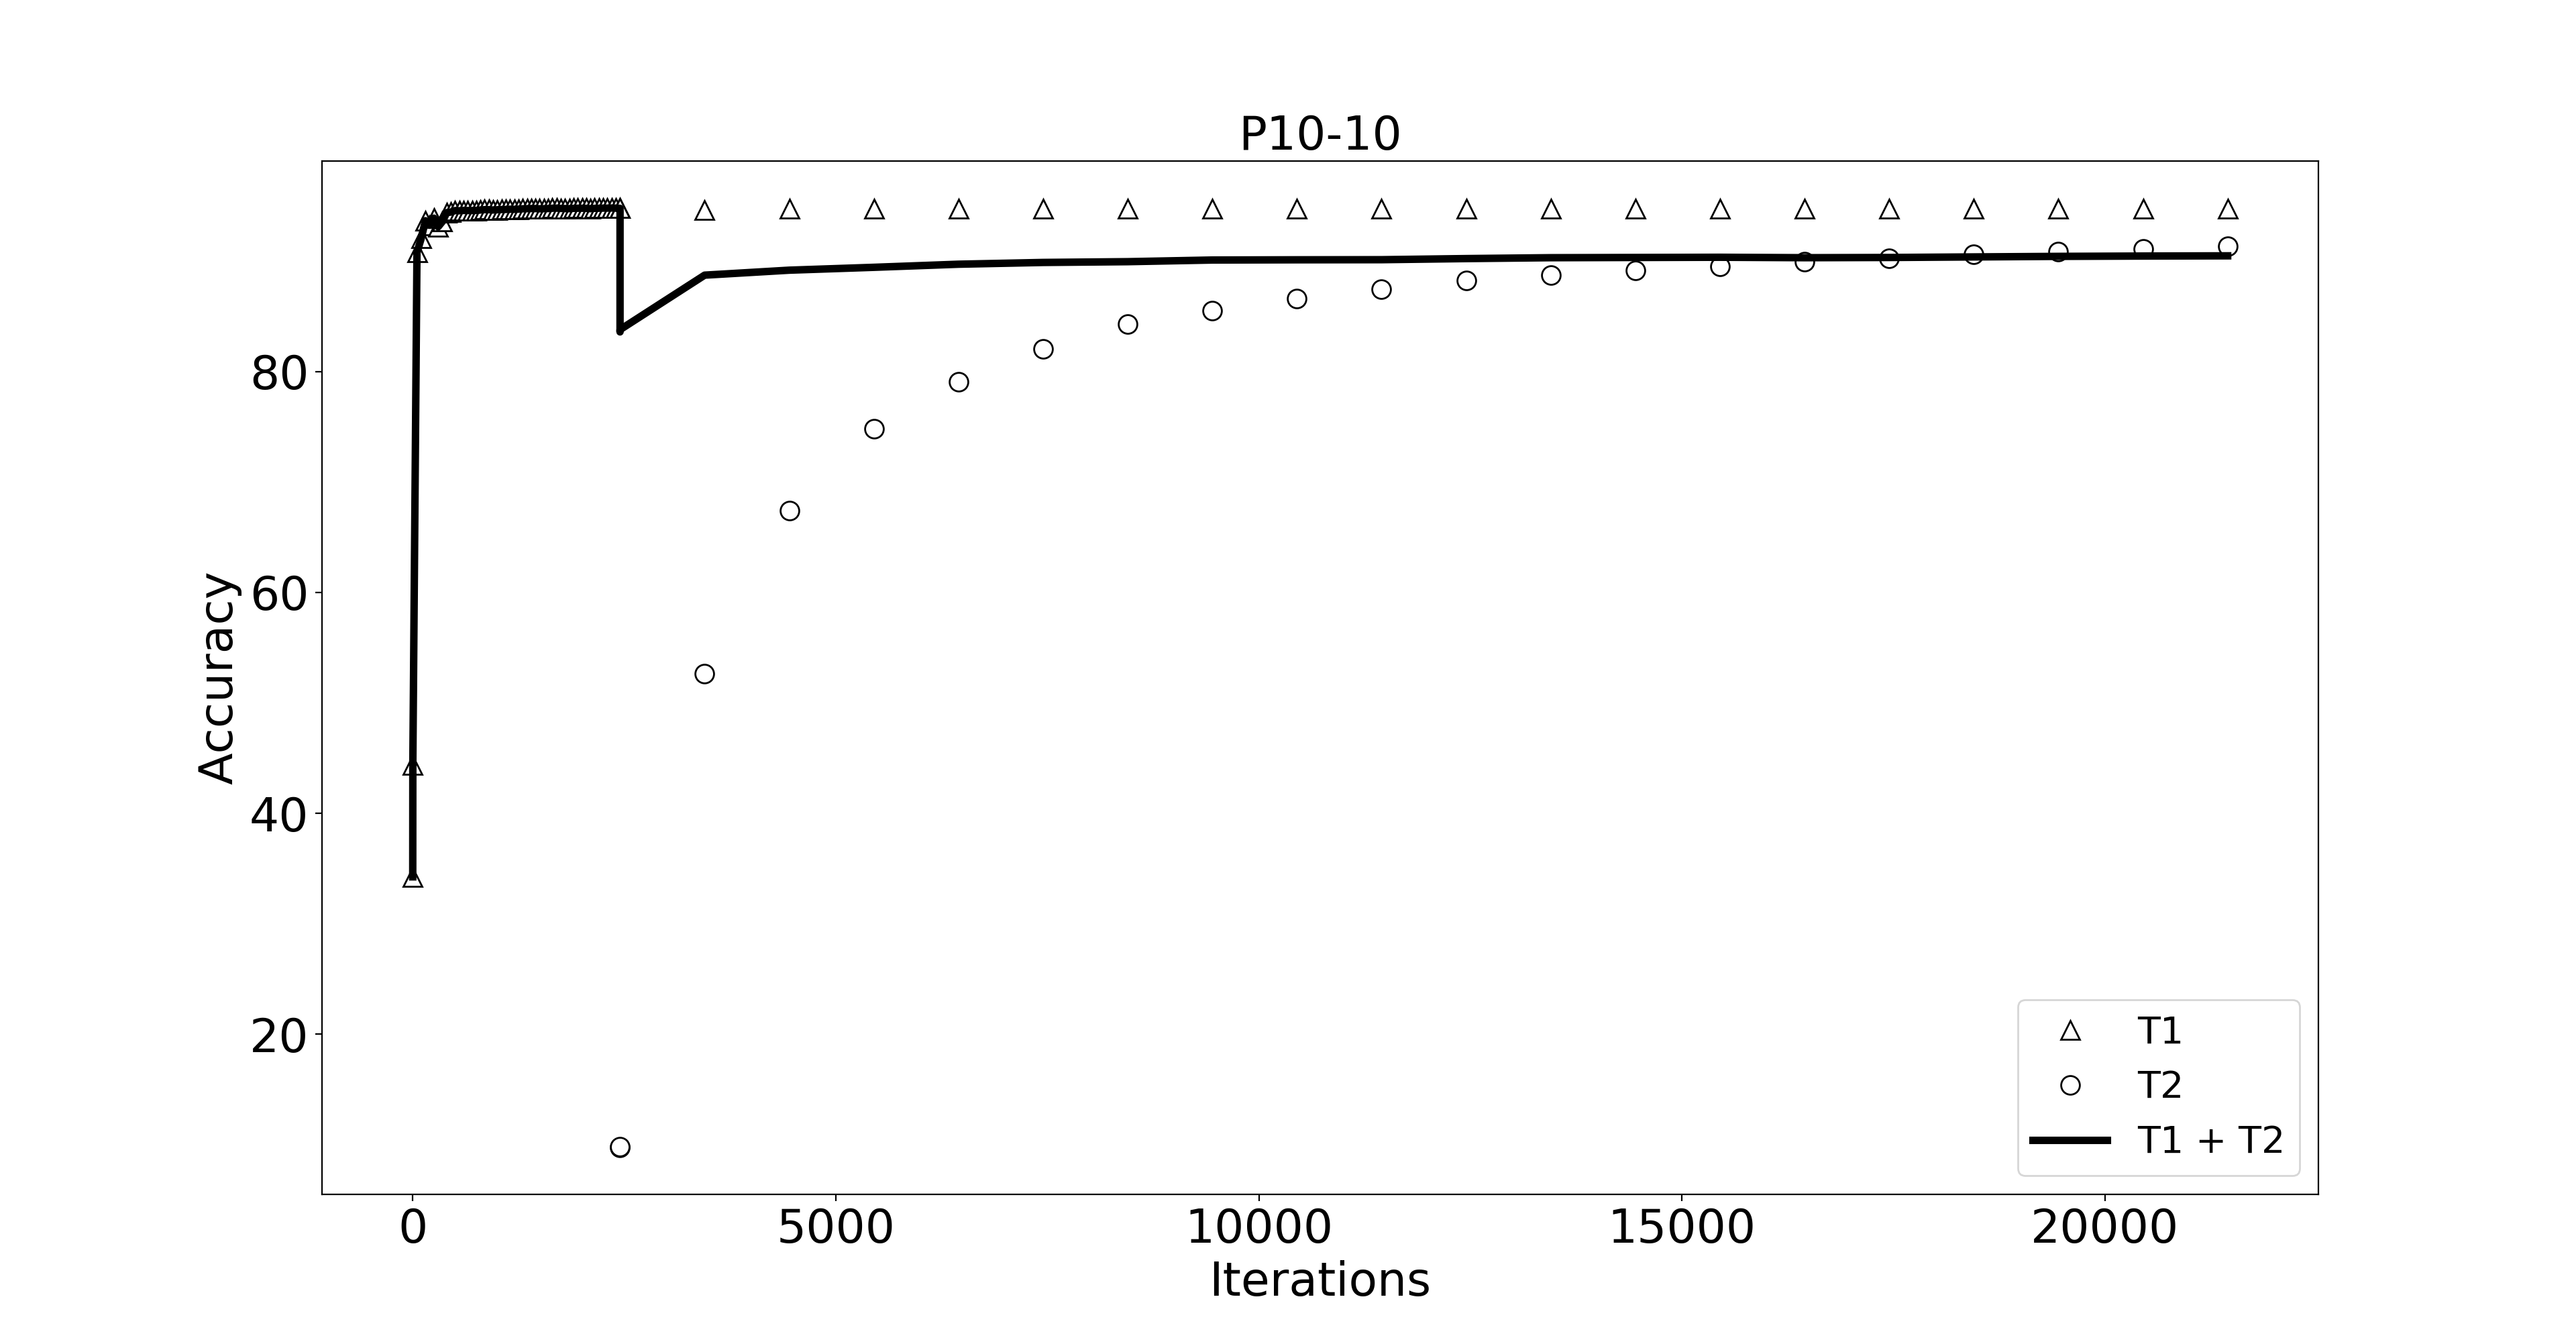
\includegraphics[width=\textwidth]{project/experiments/P10-10_BS1k_IT20k}
    \caption{P10-10}
    \label{fig:exp_p10-10}
\end{figure}

\newpage

Table \ref{table:exp_d10-10} shows the results of several experiments with the learning rate and lambda of $T_2$.
The table shows that there are many good outcomes.
The best outcomes are with the same learning rate as $T_1$ and rather small lambda value.

\begin{table}[H]
    \centering
    \begin{tabular}{ |c|l|l|l|  }
        \hline
        \multicolumn{2}{|c|}{parameters} & \multicolumn{2}{c|}{accuracy} \\
        \hline
        learning rate & lambda & $T_2$ & complete dataset\\
        \hline
        \hline
        \multirow{6}{*}{0.001} & 1,000 & 97.09\% & 93.72\%\\
                            & 10,000 & 97.66\% & 94.20\%\\
                            & 100,000 & 97.2\% & 93.05\% \\
                            & 1,000,000 & 97.3\% & 93.26\% \\
                            & 1,010,000 & 97.25\% & 92.46\% \\
                            & 1,050,000 & 96.84\% & 92.29\% \\
        \hline
        \multirow{6}{*}{0.0001} & 1,000 & 96.87\% & 91.41\%\\
                                & 10,000 & 96.51\% & 90.93\%\\
                                & 100,000 & 96.48\% & 91.45\% \\
                                & 1,000,000 & 96.45\% & 91.47\% \\
                                & 1,010,000 & 96.56\% & 91.43\% \\
                                & 1,050,000 & 96.45\% & 91.38\% \\
        \hline
        \multirow{6}{*}{0.00001} & 1,000 & 94.67\% & 90.98\%\\
                                & 10,000 & 93.04\% & 90.67\%\\
                                & 100,000 & 91.53\% & 90.46\% \\
                                & 1,000,000 & 90.29\% & 90.66\% \\
                                & 1,010,000 & 90.28\% & 90.65\% \\
                                & 1,050,000 & 90.23\% & 90.66\% \\
        \hline
        \multirow{6}{*}{0.000001} & 1,000 & 87.84\% & 89.75\% \\
                                & 10,000 & 80.58\% & 89.67\% \\
                                & 100,000 & 68.64\% & 89.17\% \\
                                & 1,000,000 & 56.66\% & 88.64\% \\
                                & 1,010,000 & 56.62\% & 88.63\% \\
                                & 1,050,000 & 56.51\% & 88.62\% \\
        \hline
    \end{tabular}
    \caption{Experiment P10-10}
    \label{table:exp_d10-10}
\end{table}
